\subsection{SDK}

\subsubsection{Creazione di un widget immagine}

\label{Creazione di un widget immagine}
\begin{figure}[ht]
	\centering
	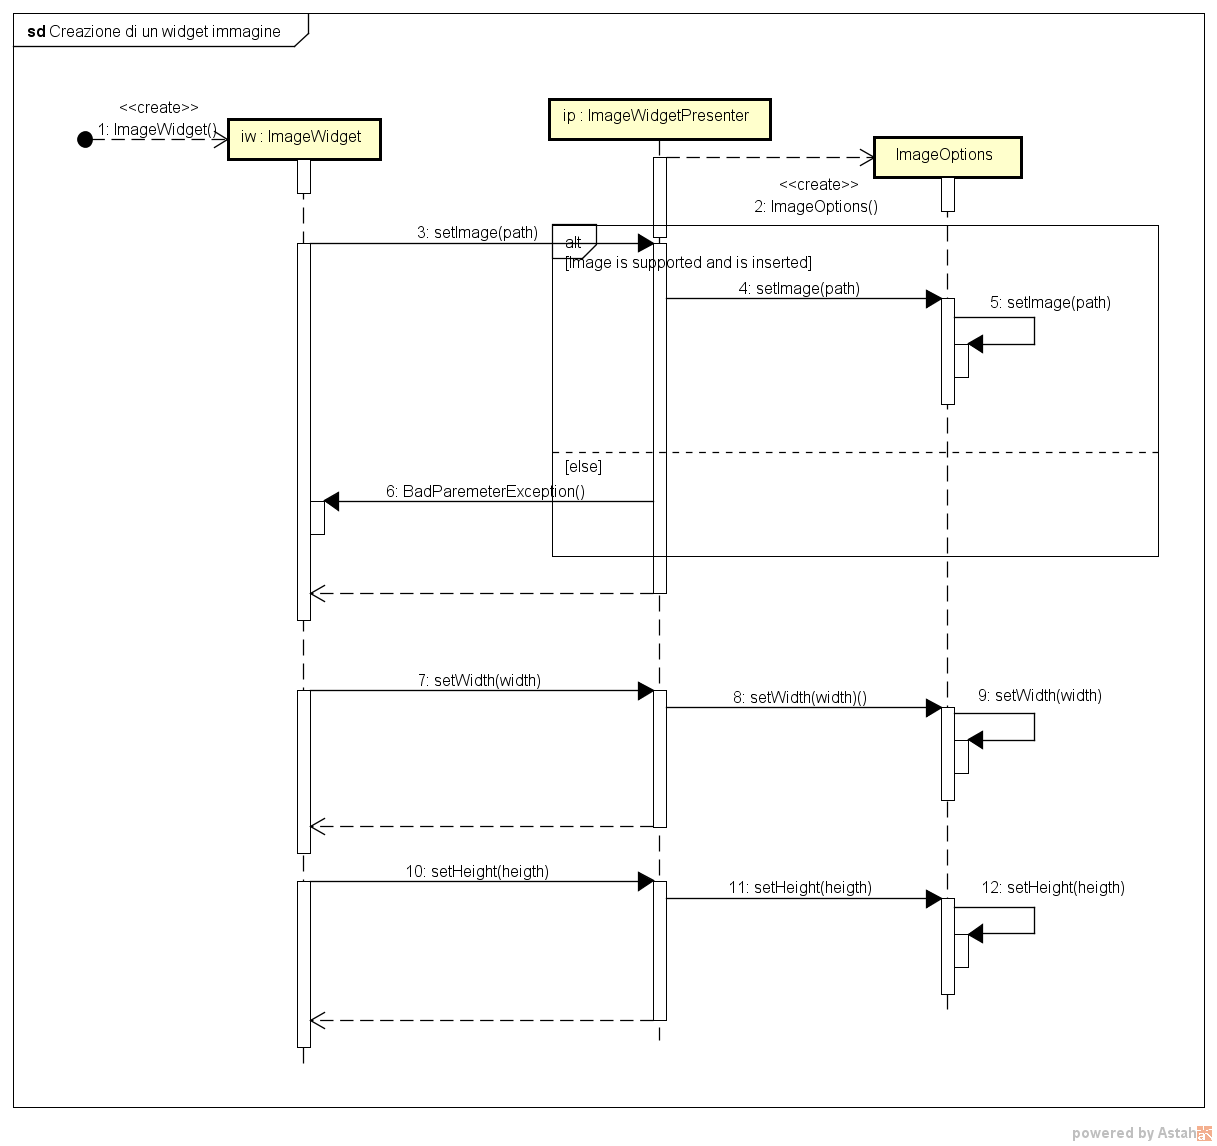
\includegraphics[width=16cm, height=14cm]{Sezioni/Diagrammi/img/Creazione di un widget immagine.png}
	\caption{Creazione di un widget immagine}
\end{figure}

Lo sviluppatore può creare un widget di tipo immagine per aggiungerlo ad una sua ipotetica \termine{bolla}. Durante la costruzione, come si vede dallo schema, vengono invocati dei metodi. Il primo per impostare l'immagine e gli altri due per impostare larghezza ed altezza rispettivamente. Il tipo delle immagini supportate sono le stesse supportate da \termine{Rocket Chat} ovvero:
\begin{itemize}
\item .jpeg
\item .gif
\item .png
\item .jpg
\end{itemize}
Se l'immagine inserita non appartiene ad uno di questi formati oppure non viene inserita dallo sviluppatore il metodo \texttt{setText} di \texttt{TextWidgetPresenter} lancerà un'eccezione di tipo \texttt{BadParameterException}.
Le frecce di ritorno dal \texttt{ImageWidgetPresenter} al \texttt{ImageWidget} sono state inserite poiché il cambiamento dei dati sul Presenter ha effetto anche sulla View. La comunicazione tra queste due unità avviene tramite il \termine{framework} \termine{vue.js}.
Si noti, infine, che i metodi invocati da \texttt{ImageWidget} vengono chiamati in quest'ordine dal suo costruttore senza parametri. Tali metodi possono anche essere chiamati singolarmente dallo sviluppatore secondo l'ordine che egli preferisce. Queste azioni non verranno ulteriormente descritte poiché ritenute ridondanti.

\newpage

\subsubsection{Creazione di un widget di testo}

\label{Creazione di un widget di testo}
\begin{figure}[ht]
	\centering
	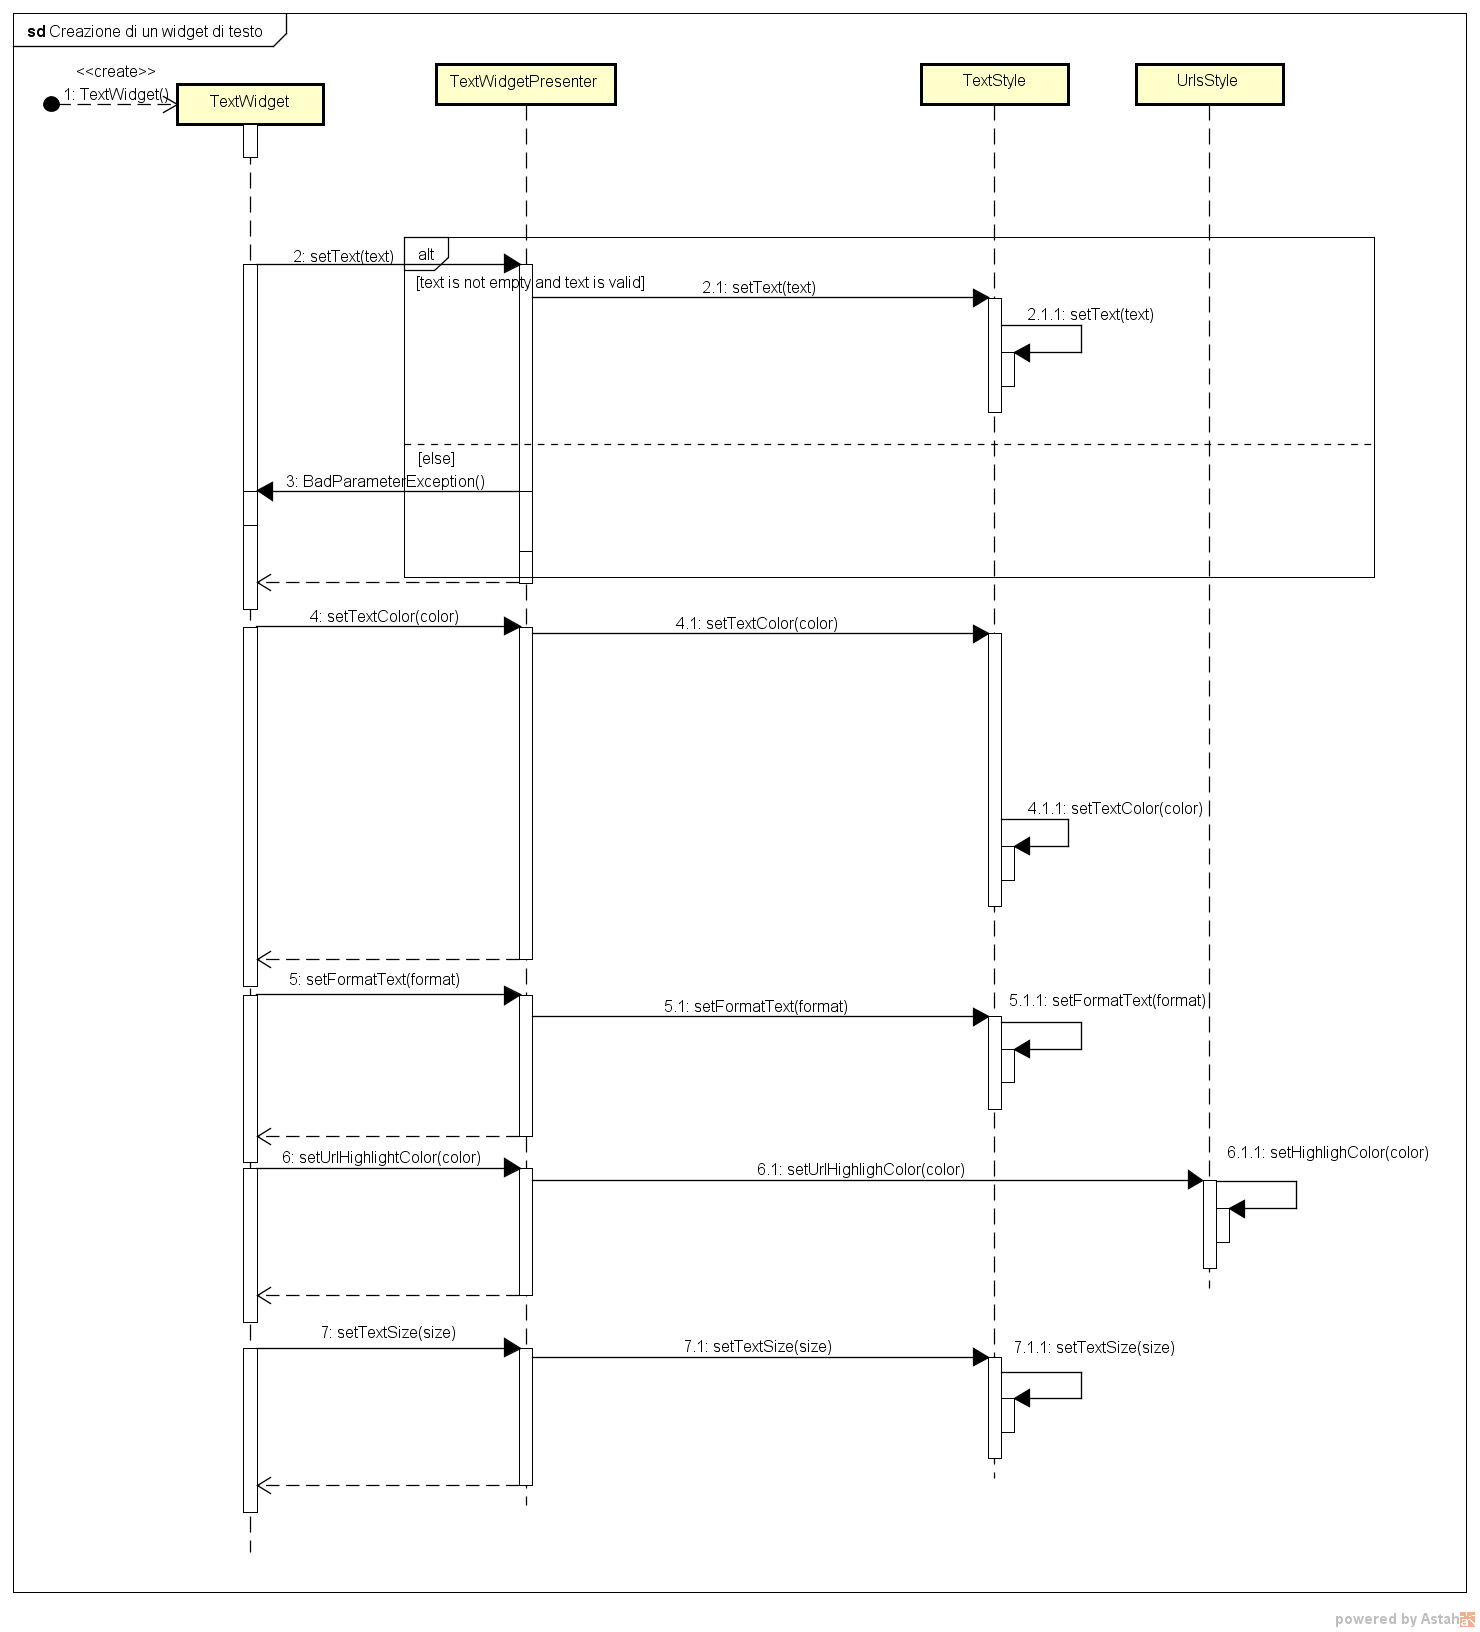
\includegraphics[width=16cm, height=14cm]{Sezioni/Diagrammi/img/Creazione di un widget di testo.png}
	\caption{Creazione di un widget di testo}
\end{figure}

Lo sviluppatore può creare un widget di tipo testo per aggiungerlo ad una sua ipotetica \termine{bolla}. Affinché non si verifichino errori il testo inserito nel widget deve essere valido, ovvero non deve contenere caratteri speciali se non quelli per il \termine{markdown} e non deve essere del testo vuoto. Se ciò dovesse capitare il metodo \texttt{setText} di \texttt{TextWidgetPresenter} lancerà un'eccezione di tipo \texttt{BadParameterException}.
Le frecce di ritorno dal \texttt{TextWidgetPresenter}  al \texttt{TextWidget} sono state inserite poiché il cambiamento dei dati sul Presenter ha effetto anche sulla View. La comunicazione tra queste due unità avviene tramite il \termine{framework} \termine{vue.js}.
Si noti, infine, che i metodi invocati da \texttt{TextWidget} vengono chiamati in quest'ordine dal suo costruttore senza parametri. Tali metodi possono anche essere chiamati singolarmente dallo sviluppatore secondo l'ordine che egli preferisce. Queste azioni non verranno ulteriormente descritte poiché ritenute ridondanti.

\newpage

\subsubsection{Creazione di un widget Checklist}

\label{Creazione di un widget Checklist}
\begin{figure}[ht]
	\centering
	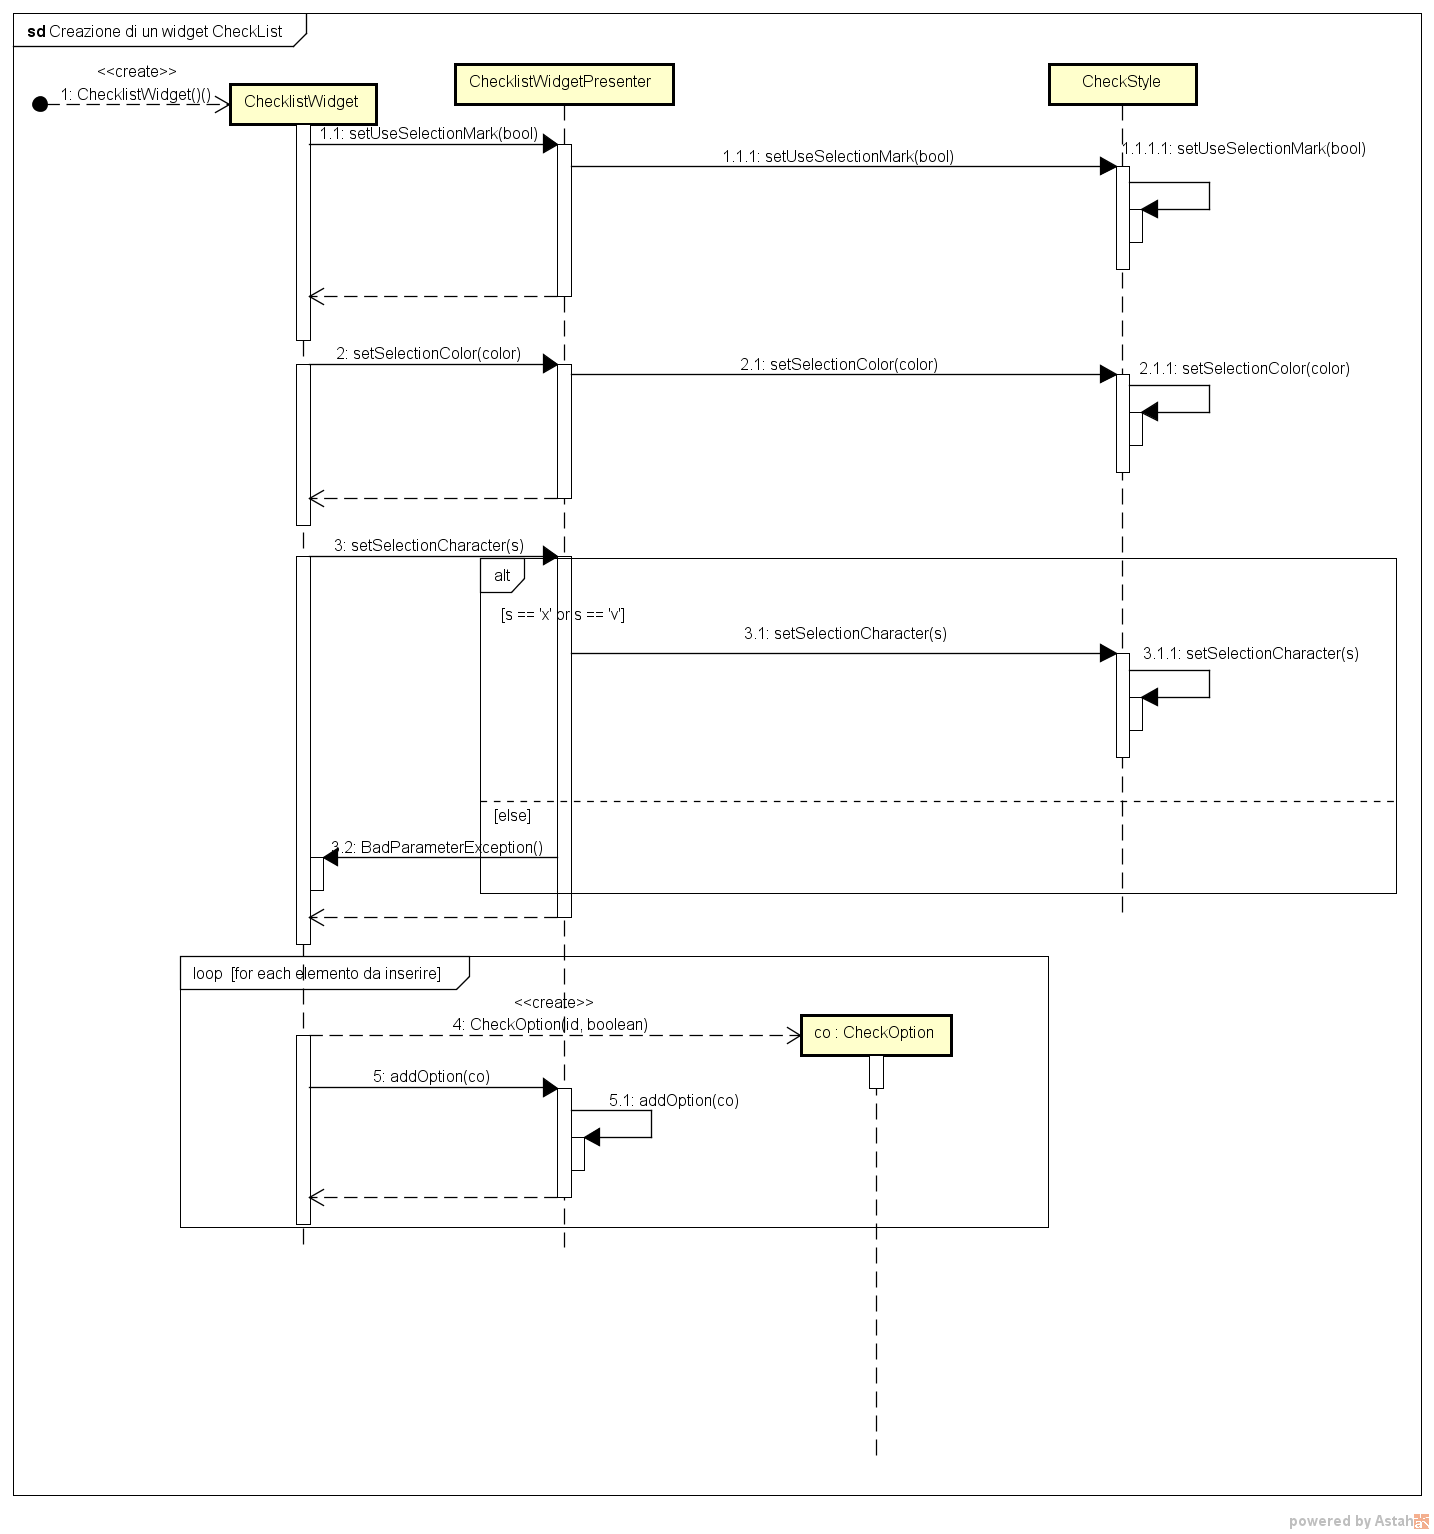
\includegraphics[width=16cm, height=14cm]{Sezioni/Diagrammi/img/Creazione di un widget CheckList.png}
	\caption{Creazione di un widget Checklist}
\end{figure}

Lo sviluppatore può creare un widget di tipo Checklist per aggiungerlo ad una sua ipotetica \termine{bolla}. Affinché non si verifichino errori, quando si usa il metodo \texttt{setSelectionCharacter} deve essere inserito correttamente un carattere per la spunta supportato. Inoltre se il flag \texttt{useSelectionMark} è stato impostato a false allora, indipendentemente dal carattere scelto dalla spunta, verrà usato il colore.
Le frecce di ritorno dal \texttt{ChecklistWidgetPresenter}  al \texttt{ChecklistWidget} sono state inserite poiché il cambiamento dei dati sul Presenter ha effetto anche sulla View. La comunicazione tra queste due unità avviene tramite il \termine{framework} \termine{vue.js}.
Si noti, infine, che i metodi invocati da \texttt{Checklist} vengono chiamati in quest'ordine dal suo costruttore senza parametri. Tali metodi possono anche essere chiamati singolarmente dallo sviluppatore secondo l'ordine che egli preferisce. Queste azioni non verranno ulteriormente descritte poiché ritenute ridondanti.

\newpage

\subsubsection{Aggiungere un messaggio di completamento al widget Checklist}

\label{Aggiungere un messaggio di completamento al widget Checklist}
\begin{figure}[ht]
	\centering
	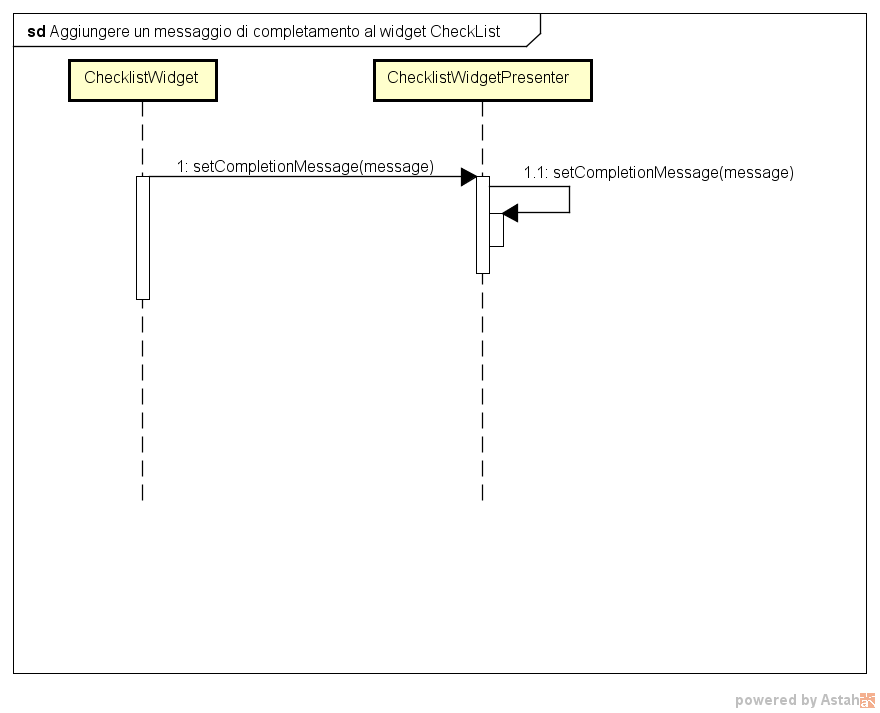
\includegraphics[width=16cm, height=14cm]{Sezioni/Diagrammi/img/Aggiungere un messaggio di completamento al widget Checklist.png}
	\caption{Aggiungere un messaggio di completamento al widget Checklist}
\end{figure}

Lo sviluppatore può aggiungere un messaggio di completamento per il widget Checklist. Questo messaggio verrà visualizzato non appena tutte le entry del widget saranno spuntate, ovvero al lancio dell'evento \texttt{emitOnCompletedList}.

\newpage

\subsubsection{Creazione di un widget bottone}

\label{Creazione di un widget bottone}
\begin{figure}[ht]
	\centering
	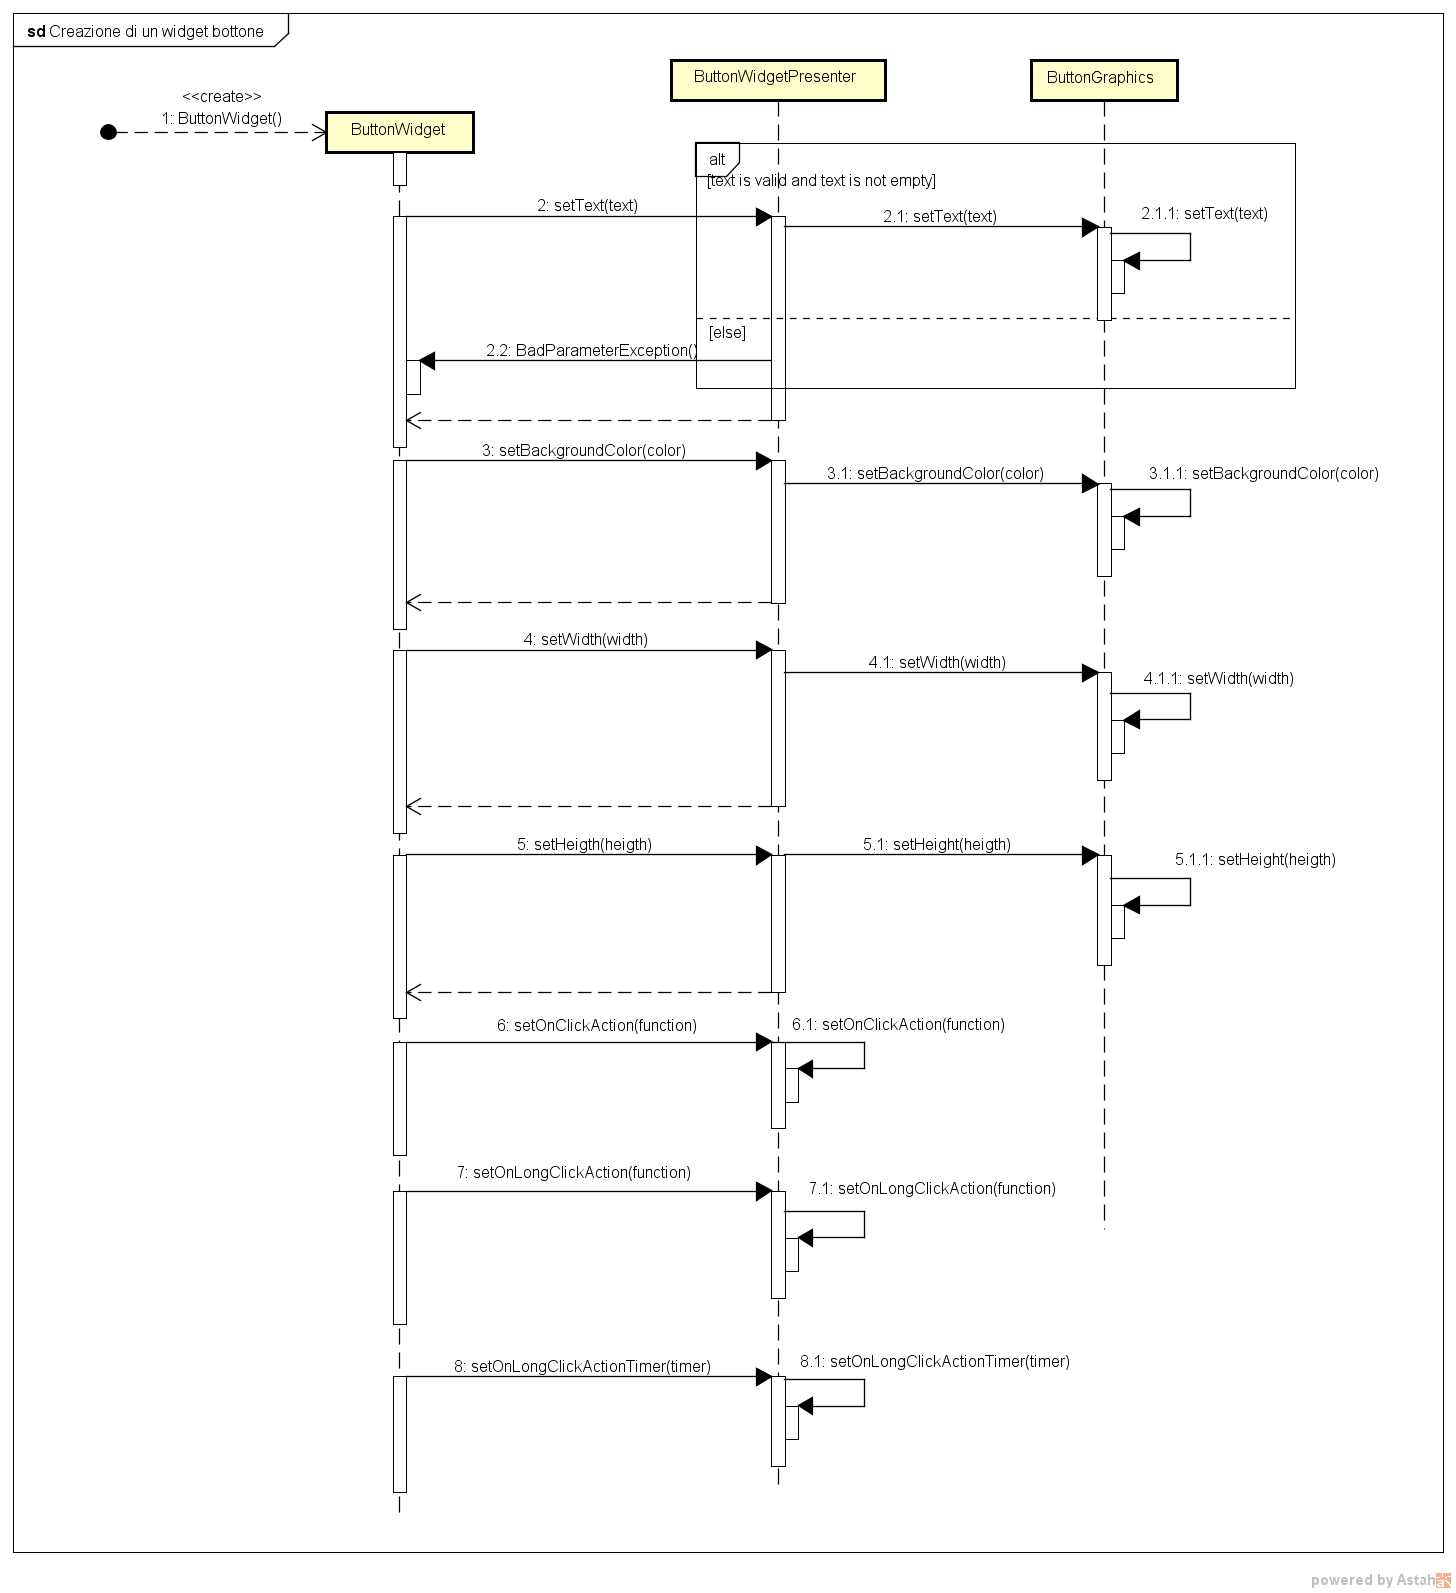
\includegraphics[width=16cm, height=14cm]{Sezioni/Diagrammi/img/Creazione di un widget bottone.png}
	\caption{Creazione di un widget bottone}
\end{figure}

Lo sviluppatore può creare un widget di tipo bottone per aggiungerlo ad una sua ipotetica \termine{bolla}. Se, durante la creazione del widget, il testo non dovesse essere impostato correttamente il metodo \texttt{setText} di \texttt{ButtonWidgetPresenter} lancerà un'eccezione di tipo \texttt{BadParameterException}.
Le frecce di ritorno da \texttt{ButtonWidgetPresenter}  a \texttt{ButtonWidget} sono state inserite poiché il cambiamento dei dati sul Presenter ha effetto anche sulla View. La comunicazione tra queste due unità avviene tramite il \termine{framework} \termine{vue.js}.
Si noti, infine, che i metodi invocati da \texttt{ButtonWidget} vengono chiamati in quest'ordine dal suo costruttore senza parametri. Tali metodi possono anche essere chiamati singolarmente dallo sviluppatore secondo l'ordine che egli preferisce. Queste azioni non verranno ulteriormente descritte poiché ritenute ridondanti.

\newpage

\subsubsection{Creazione di un listWidget}

\label{Click di un bottone}
\begin{figure}[ht]
	\centering
	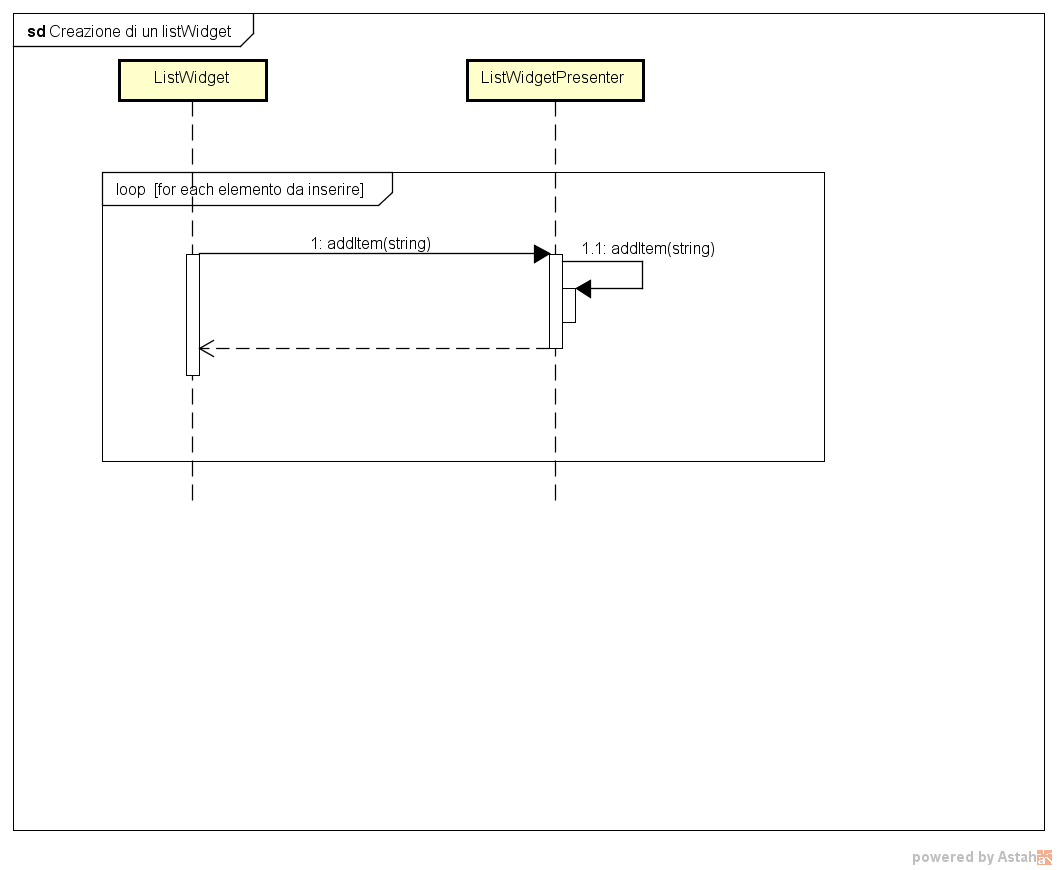
\includegraphics[width=16cm, height=14cm]{Sezioni/Diagrammi/img/Creazione di un listWidget.png}
	\caption{Creazione di un listWidget}
\end{figure}

Lo sviluppatore può creare un widget di tipo lista per aggiungerlo ad una sua ipotetica \termine{bolla}. Ogni elemento aggiunto logicamente dal presenter agisce anche sulla view. Per questo tipo di comunicazione si rimanda al \termine{framework} \termine{vue.js}.
L'azione compiuta per creare il widget può essere anche effettuata a posteriori della creazione del widget, questa però, essendo molto simile a quella appena descritta, viene omessa per ridondanza.

\newpage

\subsubsection{Creazione di una bolla aggiungendo un widget checklist}

\label{Creazione di una bolla aggiungendo un widget checklist}
\begin{figure}[ht]
	\centering
	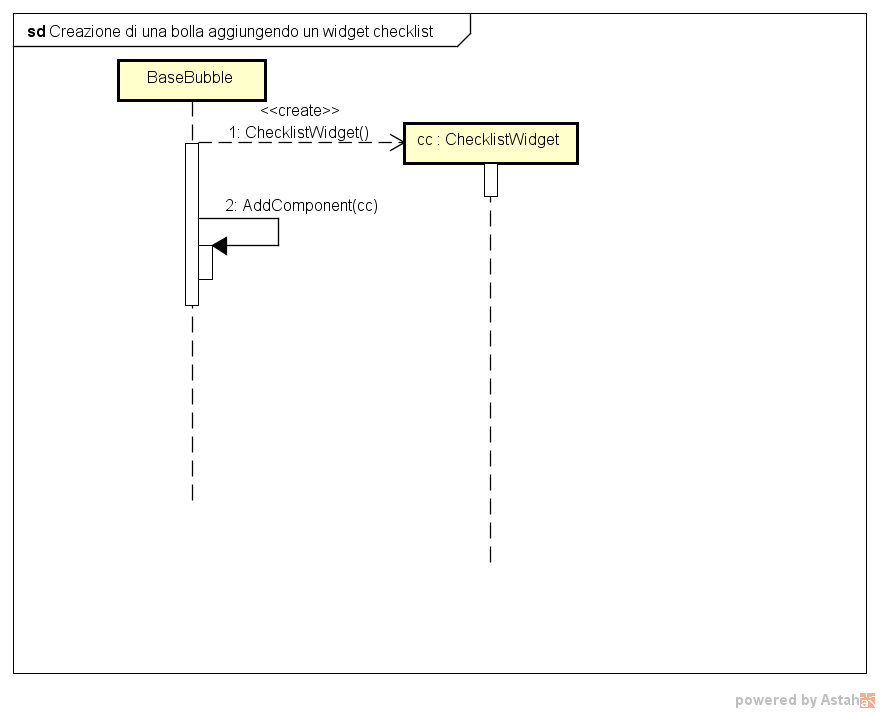
\includegraphics[width=16cm, height=14cm]{Sezioni/Diagrammi/img/Creazione di una bolla aggiungendo un widget checklist.png}
	\caption{Creazione di una bolla aggiungendo un widget checklist}
\end{figure}

Lo sviluppatore può aggiungere un widget alla \termine{bolla} appena creata. L'aggiunta dell'elemento avviene tramite il metodo \texttt{addComponent} che permette l'aggiunta sia di un layout che di un widget. Si noti che l'esempio è fatto con un widget specifico, ovvero il widget checklist, ma ciò vale per qualsiasi widget presente nell'\termine{SDK}. Gli altri esempi simili vengono, per questo motivo, omessi.

\newpage

\subsubsection{Aggiunta ad una bolla di un Layout contenente due widget di testo}

\label{Aggiunta ad una bolla di un Layout contenente due widget di testo}
\begin{figure}[ht]
	\centering
	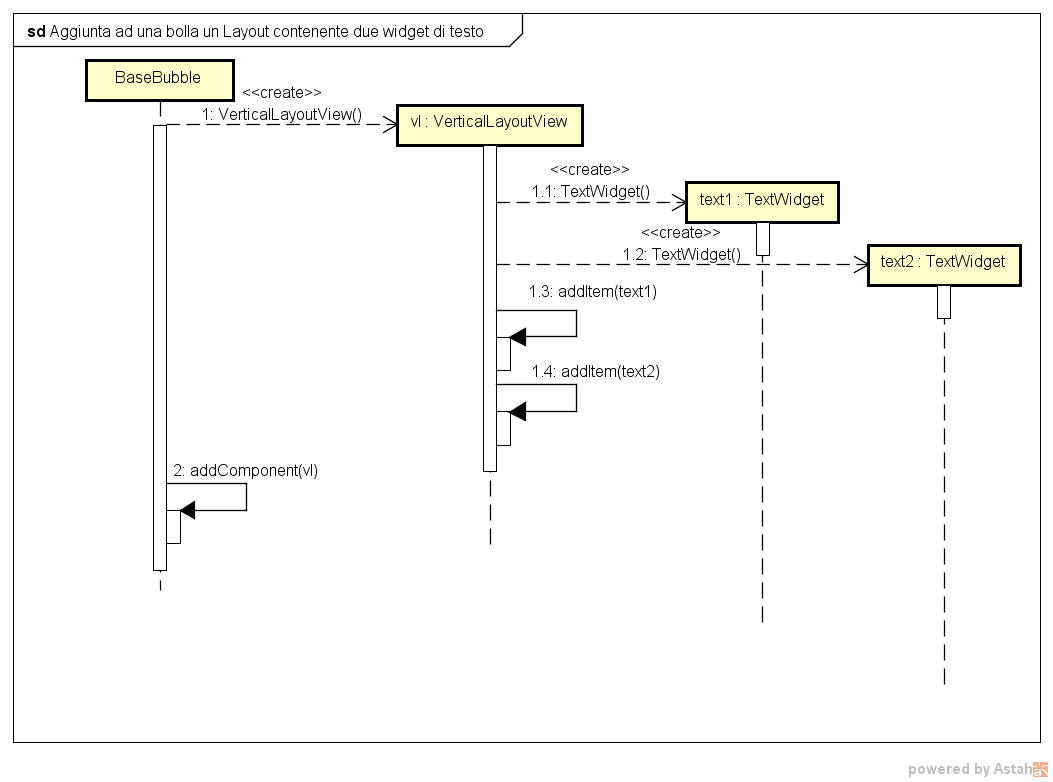
\includegraphics[width=16cm, height=14cm]{Sezioni/Diagrammi/img/Aggiunta ad una bolla un Layout contenente due widget di testo.png}
	\caption{Aggiunta ad una bolla di un Layout contenente due widget di testo}
	
\end{figure}
Lo sviluppatore può aggiungere un layout contenente dei widgets alla \termine{bolla}. Anche questo rappresenta solo un generico esempio di come si possa aggiungere un layout ad una \termine{bolla}. Gli altri esempi simili saranno, dunque, omessi. 

\newpage

\subsubsection{Creazione di una bolla MarkDownBubble}

\label{Creazione di una bolla MarkDownBubble}
\begin{figure}[ht]
	\centering
	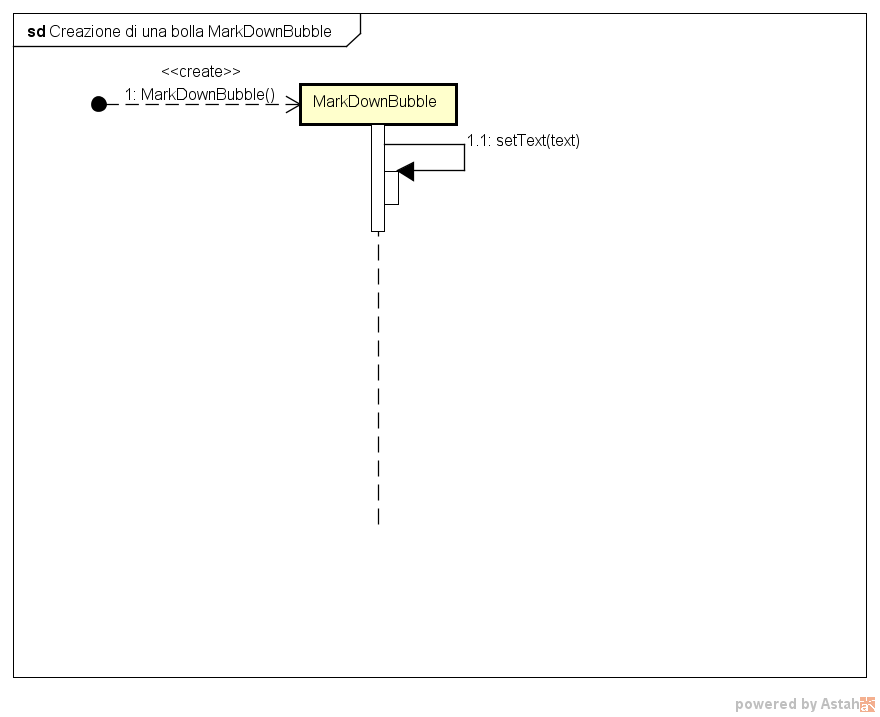
\includegraphics[width=12cm, height=8cm]{Sezioni/Diagrammi/img/Creazione di una bolla MarkDownBubble.png}
	\caption{Creazione di una bolla MarkDownBubble}
	
\end{figure}

Lo sviluppatore può creare una \termine{bolla} MarkDownBubble disponibile nell'\termine{SDK}.

\subsubsection{Creazione di una bolla AlertBubble}

\label{Creazione di una bolla AlertBubble}
\begin{figure}[ht]
	\centering
	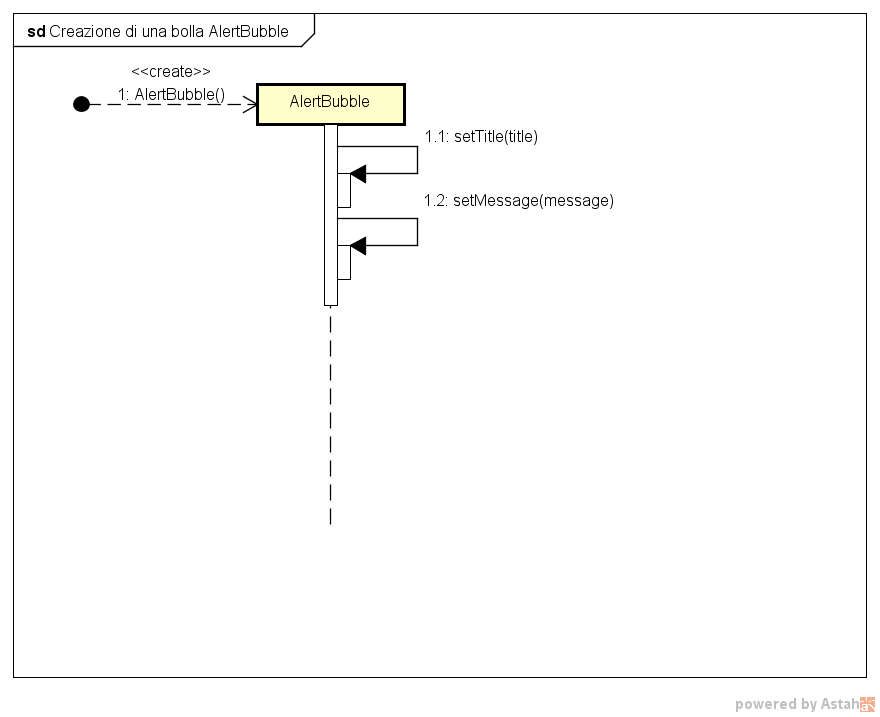
\includegraphics[width=12cm, height=8cm]{Sezioni/Diagrammi/img/Creazione di una bolla AlertBubble.png}
	\caption{Creazione di una bolla AlertBubble}
	
\end{figure}

Lo sviluppatore può creare una \termine{bolla} AlertBubble disponibile nell'\termine{SDK}.

\newpage

\subsubsection{Creazione di una bolla ToDoListBubble}

\label{Creazione di una bolla ToDoListBubble}
\begin{figure}[ht]
	\centering
	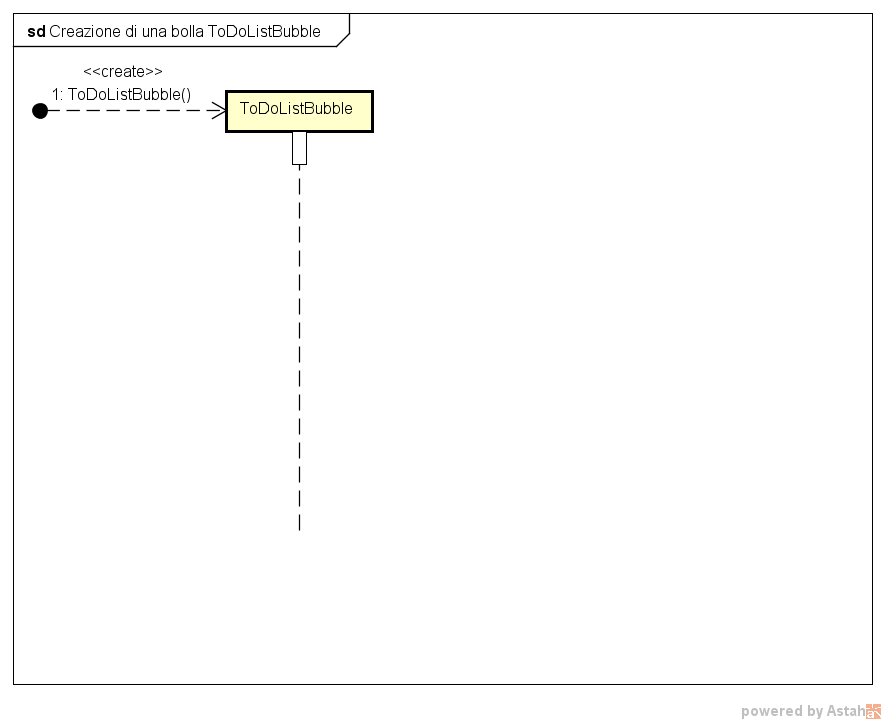
\includegraphics[width=12cm, height=8cm]{Sezioni/Diagrammi/img/Creazione di una bolla ToDoListBubble.png}
	\caption{Creazione di una bolla ToDoListBubble}
	
\end{figure}

Lo sviluppatore può creare una \termine{bolla} ToDoListBubble disponibile nell'\termine{SDK}.


